\documentclass[parskip=full,11pt,twoside]{scrartcl}
\usepackage[utf8]{inputenc}

\title{VIPER: Viper Interactive Prolog Education Runtime}
\author{Paul Brinkmeier, Lukas Brocke, Christian Oder, Aaron Maier, Jannik Koch}

% section numbers in margins:
\renewcommand\sectionlinesformat[4]{\makebox[0pt][r]{#3}#4}

% header & footer
\usepackage{scrlayer-scrpage}
\lofoot{\today}
\refoot{\today}
\pagestyle{scrheadings}

\usepackage{amsmath} % for $\text{}$

\usepackage[sfdefault,light]{roboto}
\usepackage[T1]{fontenc}
\usepackage[german]{babel}
\usepackage[yyyymmdd]{datetime} % must be after babel
\renewcommand{\dateseparator}{-} % ISO8601 date format
\usepackage{hyperref}
\usepackage[nameinlink]{cleveref}
\crefname{figure}{Abb}{Abb}
\usepackage[section]{placeins}
\usepackage{xcolor}
\usepackage{graphicx}
\usepackage{listings}
\usepackage{courier}
\hypersetup{
	pdftitle={Pflichtenheft},
	bookmarks=true,
}
\usepackage{csquotes}

\newcommand\urlpart[2]{$\underbrace{\text{\texttt{#1}}}_{\text{#2}}$}

\usepackage{pflichtenheft}

\lstset{basicstyle=\ttfamily,breaklines=true}

\begin{document}
\maketitle
\newpage

\section{Einleitung}

Prolog ist eine logische Programmiersprache die ein deklaratives Programmieren ermöglicht.

Das Grundprinzip von Prolog operiert auf einer Wissensdatenbank, deren Einträge sich Fakten und Regeln nennen.

\begin{lstlisting}
father(abe, homer).
father(homer, bart).
\end{lstlisting}

So gilt, dass Abe der Vater von Homer und Homer der Vater von Bart ist.

Dabei existiert keine Semantik.

\begin{lstlisting}
x(y, z).
a(b, c).
\end{lstlisting}

Ist eine ebenso legitime Definition.

Für eine Abfrage erhalten wir folgende Lösungen:

\begin{lstlisting}
?- father(homer, bart).
yes .
?- father(bart, abe).
no .
\end{lstlisting}

Nun ist es möglich Relationen, basierend auf Fakten, einzuführen. Definieren wir also Großvater als alle Väter von Vätern, indem wir Variablen als Platzhalter verwenden. Diese beginnen mit Großbuchstaben, Funktoren und Atome mit Kleinbuchstaben.

\begin{lstlisting}
grandfather(X, Y) :- father(X, Z), father(Z, Y).
\end{lstlisting}

Selbiges ist möglich für Abfragen.

\begin{lstlisting}
?- father(X, bart).
X = homer .
?- father(X, Y).
X = homer, Y = bart ;
X = abe, Y = homer .
?- grandfather(X, Y).
X = abe, Y = bart .
\end{lstlisting}

Die Antworten sind alle möglichen Kombinationen aus den Variablen, die den Fakten und Relationen entsprechen.

Prolog ist hierbei anders als \enquote{andere} Programmiersprachen, da es sich um eine deklarative Programmiersprache handelt. Die Relationen basieren auf zuvor definierten Fakten.

VIPER, die VIPER Interactive Prolog Education Runtime, ist ein Programm zur Bearbeitung und dem Testen von einfachen Prolog-Programmen. Über die visuelle Schnittstelle ist es dem Nutzer möglich, Prolog zu schreiben, Abfragen zu stellen und diese visualisieren zu lassen.

Dank des automatisch generierten Graphen ist es dem Nutzer hierbei möglich, die Interpretation des Programmes schrittweise anzuzeigen und nachzuvollziehen.

Damit soll dem Nutzer die Funktionsweise von Prolog-Programmen durch die graphische Visualisierung näher gebracht und zum verbesserten Verständnis von Prolog beigetragen werden.

\pagebreak
\section{Kriterien}
% Diese Section sollte kurz und knapp "für Manager" sein
% und auf eine Seite passen.

\subsection{Muss}

\criterium{Erstellen}{crt:new}

Das Programm soll in der Lage dazu sein, neue Prolog-Programme anzulegen.

\criterium{Öffnen}{crt:open}

Das Programm soll bereits vorhandene Prolog-Programme öffnen können, damit auf diesen Abfragen durchgeführt und diese visualisiert werden können.

\criterium{Speichern}{crt:save}

Das Programm soll Änderungen am momentan geöffnetem Prolog-Programm speichern können. Wurde die Datei seit dem Öffnen anderweitig verändert, so wird sie überschrieben.

\criterium{Parsen eines Prolog-Programms mit begrenztem Umfang}{crt:parser}

% Verweis auf Glossareintrag
Das Programm kann eine Teilmenge der Sprache Prolog durch einen Parser verarbeiten:

Es gibt IDs, Variablen und Zahlen die wie folgt notiert werden:

\begin{lstlisting}
id := [a-z][a-zA-Z0-9]*
var := [A-Z][a-zA-Z0-9]*
num := [0-9]*
\end{lstlisting}

Es gibt Terme welche sich aus obigem zusammensetzen:

\begin{lstlisting}
Term := Funktor | var | num
Funktor := id | id( Term{, Term}* )
\end{lstlisting}

Und zusätzlich gibt es Regeln und Ziele welche sich wie folgt zusammensetzen:

\begin{lstlisting}
Regel := Funktor . | Funktor :- Ziel {, Ziel}* .
Ziel := Funktor | Term = Term
\end{lstlisting}

Eine Regel die nur aus einem Funktor ohne Ziel besteht wird Fakt genannt.

Das Programm unterstützt die Darstellung von Listen. Die leere Liste wird durch \enquote{\texttt{[]}} dargestellt, eine Liste mit Inhalt wird durch \enquote{\texttt{[1,2,3]}} dargestellt und intern als Listenkopf und \enquote{Restliste} behandelt, das heißt:\newline
Liste: \texttt{[1,2,3]}\newline
In Prolog: \texttt{[1|teilliste1]}, \texttt{teilliste1=[2|teilliste2]}, \texttt{teilliste2=[3]}.

\criterium{Einzelschritt-Interpreter}{crt:interpreter}

% Verweis auf GUI und mögliche Anpassung des Schaltflächennamen
Das Programm bearbeitet Anfragen schrittweise. Nach jedem durchgeführten Teilschritt einer Abfrage wartet das Programm auf Interaktion vom Nutzer (drücken der Verarbeiten-Schaltfläche), bis es den nächsten Teilschritt bearbeitet.

\criterium{Visualisierung}{crt:visualization}

% Verweise auf GUI
Das Programm kann Abfragen zu einem Prolog-Programm mit Hilfe eines Graphen visualisieren. Dieser hat eine Baumstruktur und beinhaltet für jeden Abarbeitungsschritt einen eigenen Knoten.

\subsection{Kann}

\criteriumOptional{Zurückschreiten}{crt:stepback}

% Verweis auf GUI
Das Programm soll es dem Nutzer ermöglichen, beliebig viele Schritte schrittweise zurückzugehen.

\criteriumOptional{Ausführung bis zur nächsten Ausgabe}{crt:continue}

% Verweis auf GUI
Die Interpretation soll durch eine zusätzliche Schaltfläche bis zur nächsten Ausgabe ausgeführt werden können.

\criteriumOptional{Abbrechen}{crt:cancel}

% Verweis auf GUI
Das automatische Abarbeiten mehrerer Schritte soll durch das Betätigen einer Schaltfläche abgebrochen werden können.

\criteriumOptional{Cut}{crt:cut}

Das Programm soll die \enquote{Cut}-Funktionalität unterstützen. Mit dieser kann der Nutzer dem Interpreter durch das hinzufügen eines \enquote{\texttt{!}} als Teilziel verbieten zu einer bestimmten Stelle zurück zu springen.

\criteriumOptional{Arithmetik}{crt:maths}

Das Programm soll grundlegende Arithmetik unterstützen. Da Terme in Prolog nur für sich selber stehen, können Abfragen wie \enquote{$4 = 1 + 3$} nicht bearbeitet werden. Daher wird der Interpreter um ein Rechenoperator \enquote{\texttt{is}} erweitert, welcher solche arithmetischen Abfragen ermöglicht.

\criteriumOptional{Standardbibliothek}{crt:standardlib}

Das Programm soll eine Standardbibliothek in Form eines Prolog-Programms mit nützlichen, vordefinierten Regeln unterstützen, die standardmäßig beim Starten des Programms mit eingebunden wird.

\criteriumOptional{Standardbibliothek deaktivieren}{crt:disablelib}

Das Programm soll es dem Nutzer ermöglichen, die eingebundene Standardbibliothek deaktivieren zu können.

\criteriumOptional{Export von Visualisierungsbäumen als LaTeX-Code}{crt:latexexport}

Das Programm kann einen Visualisierungsbaum als LaTeX-Code exportieren, damit dieser vereinfacht in Dokumente eingebunden werden kann.

\criteriumOptional{Export von Visualisierungsbäumen als Bilddatei}{crt:imageexport}

Das Programm kann einen Visualisierungsbaum als Bilddatei im SVG- oder PNG-Format exportieren.

\criteriumOptional{Syntax-Highlighting}{crt:syntaxhighlighting}

Das Programm soll das farbliche Hervorheben bestimmter Regeln und ihres/ihrer korrespondieren Knoten in der Visualisierung unterstützen. Der Code wird dabei farblich passend hervorgehoben. Identifier und Variablen werden unterschiedlich zu Zahlen eingefärbt. Ebenfalls unterscheiden sich die Farben von umschließenden Klammern. Die Operatoren \texttt{=}, \texttt{:-}, \texttt{is} und \texttt{!} sind farblich von allem anderen unterscheidbar.

\criteriumOptional{\enquote{Pretty-Printing} von Listen}{crt:prettyprinting}

Das Programm soll Listen bei der Ausgabe einheitlich auf \enquote{\texttt{[x,y,z]}} formatieren.

\criteriumOptional{Formatierung von Quelltext}{crt:formatting}

Das Programm soll Quelltext in ein vorgeschriebenes Format bringen können.

\subsection{Abgrenzung}

\criteriumNot{Voller Sprachsupport}{crt:fullsupport}

Das Programm hat kein Verständnis für Prolog-Sprachfeatures außerhalb der vorgestellten Prolog-Teilmenge.

\criteriumNot{Andere Programmiersprachen}{crt:otherlanguages}

Das Programm beschränkt sich auf die Prolog-Sprache und bietet keine offizielle Unterstützung für Prolog-Dialekte oder andere Programmiersprachen jeglicher Art.

\criteriumNot{Nutzung in einer Kommandozeile}{crt:cli}

Das Programm beschränkt sich auf eine graphische Darstellung über GUI-Elemente. Eine Interaktion über die Konsole wird nicht unterstützt.

\criteriumNot{Professionelle Anwendung}{crt:professionaluse}

Das Programm ist nicht für professionelle Anwendungszwecke ausgelegt.

\pagebreak
%%%%%%%%%%%%%%
\section{Produkteinsatz}

Das Programm soll als graphisches Prolog-Lerntool betrieben werden.

Die Zielgruppe des Lerntools sind Lehrende, Studierende und Enthusiasten.

Das Programm soll sich auf eine Teilmenge der Prolog-Sprache beschränken, diese jedoch voll unterstützen.

Das Programm soll für die Teilmenge der Sprache eine Lernhilfe sein und das Verständnis für die Funktionsweise von Prolog, mit Hilfe von schrittweiser Visualisierung, stärken.

Das Programm ermöglicht es mit Hilfe eines eingebauten Editors Prolog-Programme zu bearbeiten und zu erweitern.

\section{Produktumgebung}

Das Programm soll als graphische Applikation auf einem Desktop-System betrieben werden.

Es stehen mindestens 2 AMD64/x86 Kerne mit insgesamt 2GB shared RAM zur Verfügung.

Unterstützte Betriebssysteme sind Windows ab Version 7 und aufwärts, macOS 10.9 aufwärts sowie Ubuntu Linux 16.04.

Eine Maus sowie eine Tastatur sind als Eingabegeräte angeschlossen und funktionsfähig.

Eine Installation des Java Runtime Environments Version 8 aufwärts ist auf dem System vorhanden.

%%%%%%%%%%%
\section{Produktdaten}

\textbf{Zuletzt geöffnete Dateien} \\
Die Pfade der fünf zuletzt geöffneten Dateien werden für einen Eintrag in der Menüleiste gespeichert. Außer den oben genannten werden keinerlei Daten gespeichert.
%%%%%%%%%%%
\section{Funktionale Anforderungen}

\functionality{Erstellen eines neuen Prolog-Programms}{fnc:new}
\fulfills{crt:new}

Das Programm stellt einen Editor bereit, in dem ein leeres Prolog-Programm angelegt werden kann. Sollte der Editor zuvor bereits ungesicherten Inhalt besitzen, so wird der Nutzer aufgefordert, diesen zu speichern. Der alte Inhalt wird daraufhin verworfen und ein neues Prolog-Programm angelegt.

\functionality{Öffnen eines Prolog-Programms}{fnc:open}
\fulfills{crt:open}

Das Programm ist in der Lage, Prolog-Programmdateien zu öffnen. Der Datei-Inhalt wird dabei in den Editor geladen und angezeigt. Analog wird zur Erstellung eines neuen Prolog-Programms, falls nötig, zur Speicherung ungesicherter Inhalte aufgefordert und das alte Prolog-Programm daraufhin verworfen.

\functionality{Öffnen eines zuletzt verwendeten Prolog-Programms}{fnc:recentfiles}
\fulfills{crt:open}

Das Programm bietet einen Schnellzugriff auf bis zu fünf der zuletzt verwendeten Dateien an. Diese können analog zu F2 geöffnet werden.

\functionality{Bearbeiten eines Prolog-Programms}{fnc:editor}
\fulfills{crt:save}
\fulfills{crt:syntaxhighlighting}

Das Prolog-Programm kann im Editor bearbeitet werden. Die Änderungen werden erst beim Speichern zurückgeschrieben.

\functionality{Speichern des Editor-Inhalts}{fnc:save}
\fulfills{crt:save}

Das Programm kann den Inhalt des Editors auf die Festplatte schreiben. Wurde das Prolog-Programm bisher noch nicht gespeichert, so kann über einen Auswahldialog eine neue Datei angelegt werden. Der Inhalt der Datei wird ohne weitere Überprüfung überschrieben.

\functionality{Parsen eines Prolog-Programms}{fnc:parser}
\fulfills{crt:parser}
\fulfills{crt:standardlib}

Das geöffnete Prolog-Programm kann durch einen Parser verarbeitet werden. Wird der Parser gestartet, werden die Fenster der Konsole und der Visualisierung geleert.

\functionality{Fehlerausgabe beim Parsen eines inkorrekten Prolog-Programms}{fnc:errorcheck}
\fulfills{crt:parser}

Der Parser erkennt Fehler innerhalb des geöffneten Prolog-Programms bei der Verarbeitung. Fehlermeldungen werden über das verfügbare Konsolen-Fenster ausgegeben.

\functionality{Eingabe von Prolog-Abfragen in die Konsole}{fnc:shell}
\fulfills{crt:interpreter}

Bei erfolgreicher Verarbeitung einer fehlerfreien Datei durch den Parser erlaubt die angezeigte Konsole die Eingabe von Abfragen. Sollten erneut Änderungen an dem geöffneten Prolog-Programm stattfinden, so wird die Eingabe in die Konsole sowie jegliche Interaktion mit der Visualisierung gesperrt bis der veränderte Quelltext erneut vom Parser verarbeitet wurde.

\functionality{Interpretation von Prolog-Abfragen in der Konsole}{fnc:interpreter}
\fulfills{crt:interpreter}
\fulfills{crt:cut}
\fulfills{crt:maths}
\fulfills{crt:standardlib}
\fulfills{crt:prettyprinting}

Abfragen, welche in der Konsole eingegeben wurden, werden nach einer Bestätigung mit der Eingabe-Taste schrittweise interpretiert. Ausgaben des Interpreters werden in der Konsole angezeigt. Nach dem Betätigen der Schaltfläche wird ausschließlich der erste Interpretationsschritt durchgeführt. Der Nutzer hat die Möglichkeit, diese Interpretation über eine Schritt-Schaltfläche schrittweise fortzuführen. Fehler bei der Interpretation einer Abfrage werden über das Konsolen-Fenster ausgegeben und die weitere Verarbeitung wird abgebrochen. Syntaktische Fehler bei Abfragen werden über das Konsolen-Fenster ausgegeben und die weitere Verarbeitung wird unterbrochen.

\functionality{Visualisierung des aktuellen Interpretationsschrittes mittels eines Graphen}{fnc:visualization}
\fulfills{crt:visualization}

Bei aktiver Interpretation einer Abfrage wird eine Visualisierung für den aktuellen Interpretationsschritt generiert und im Visualisierungs-Fenster angezeigt. Sollte zuvor eine Visualisierung in diesem Fenster angezeigt worden sein, wird diese aus dem Fenster gelöscht.

\functionality{Vergrößern und Verkleinern der Visualisierung durch Schaltflächen oder das Mausrad}{fnc:zoom}
\fulfills{crt:visualization}

Über die Verwendung des Mausrads oder der Plus- und Minus-Schaltflächen lässt sich der angezeigte Ausschnitt des Visualisierungs-Graphen vergrößern oder verkleinern.

\functionality{Navigation der Visualisierung durch Bewegungen mit der Maus}{fnc:move}
\fulfills{crt:visualization}

Durch Drücken und Halten der linken Maustaste lässt sich der angezeigte Ausschnitt des Graphen bewegen, wodurch in diesem navigiert werden kann.

\functionality{Zurückschreiten während der Interpretation}{fnc:stepback}
\fulfills{crt:stepback}

Eine Rückschritt-Schaltfläche erlaubt bei Betätigung den jeweils vorhergehenden Schritt rückgängig zu machen. Im Falle des ersten Schrittes hat das Betätigen dieser Schaltfläche keinen Effekt.

\functionality{Ausführung der Interpretation bis zur nächsten Ausgabe}{fnc:continue}
\fulfills{crt:continue}

Eine Fortsetzen-Schaltfläche erlaubt bei Betätigung die Ausführung bis zur nächsten Ausgabe fortzuführen.

\functionality{Abbrechen einer Interpretation}{fnc:cancel}
\fulfills{crt:cancel}

Im Falle einer Interpretation die mehrere Schritte hintereinander ausführt (Fortsetzen bis zur nächsten Ausgabe), kann die laufende Interpretation über eine Abbrechen-Schaltfläche frühzeitig beendet werden.

\functionality{Exportieren der angezeigten Visualisierung in einem beliebigen Schritt als LaTeX-Dokument}{fnc:latexexport}
\fulfills{crt:latexexport}

Die aktuell angezeigte Visualisierung lässt sich als LaTeX-Dokument exportieren.

\functionality{Exportieren der angezeigten Visualisierung in einem beliebigen Schritt als Grafik}{fnc:imageexport}
\fulfills{crt:imageexport}

Die aktuell angezeigte Visualisierung lässt sich als Bild im PNG- oder SVG-Format exportieren.

\functionality{Deaktivierung der Standardbibliothek}{fnc:disablelib}
\fulfills{crt:disablelib}

Die automatisch eingebundene Standardbibliothek kann über eine Schaltfläche deaktiviert werden. Von der Standardbibliothek zur Verfügung gestellte Regeln werden nun nicht mehr berücksichtigt.

%TODO: Richtlinien als Liste?
\functionality{Formatierung des Quellcodes}{fnc:formatter}
\fulfills{crt:formatting}

Eine automatische Formatierung von Prolog-Quellcode ist über eine Schaltfläche möglich. Die Formatierung ist hierbei vorgegeben und kann nicht verändert werden. Die Formatierung sieht folgendes vor: Jede Regel wird in ihre eigene Zeile gelegt. Hat eine Regel mehrere Teilziele, so wird die Regelzeile nach dem \enquote{\texttt{:-}}-Operator umgebrochen und alle Teilziele werden in eigene Zeilen gelegt, welche mit zwei Leerzeichen eingerückt sind. Bereits gesetzte Leerzeilen werden beibehalten. Fehlende Leerzeichen vor und hinter dem \enquote{\texttt{:-}}-Operator sowie nach Kommata in Parameterlisten werden eingefügt.

\functionality{Wechsel der verwendeten Sprache}{fnc:translation}
\fulfills{crt:translation}

Über die Menüleiste kann die Sprache der GUI-Elemente zwischen Englisch und Deutsch gewechselt werden.

\functionality{Dynamisches Skalieren des Hauptfensters mit der Maus}{fnc:resizeable}
\fulfills{crt:resizeable}

Das Hauptfenster des Programms kann mit der Maus in der Größe verändert werden.

%%%%%%%%%%%
\newpage
\section{Nicht-Funktionale Anforderungen}

\nonFunctionality{Das Programm startet auf einem modernen System innerhalb von 30 Sekunden und ist voll einsatzbereit.}{nfc:startup}

\nonFunctionality{Ein importiertes oder geschriebenes Prolog-Programm im Umfang von maximal 100 Zeilen Code ist innerhalb von maximal 3 Sekunden geparst und einzelne Schritte werden innerhalb von 5 Sekunden visualisiert.}{nfc:timelimit}

\nonFunctionality{Das Design wirkt modern und ansprechend.}{nfc:design}

\nonFunctionality{Das Programm lässt sich ohne die manuelle Installation weiterer Programme durch das Ausführen einer .jar Datei starten.}{nfc:installation}

\nonFunctionality{Das Programm ist ohne Abhängigkeiten kleiner als 50 MiB, mit Abhängigkeiten kleiner als 200 MiB.}{nfc:filesize}

\nonFunctionality{Das Öffnen einer Prolog-Programmdatei mit einer Größe von unter 1 MiB geschieht in unter 5 Sekunden.}{nfc:loadfile}

\nonFunctionality{Fehlerhafte Prolog-Programme sollen nie zu einem Absturz des Programms führen.}{nfc:crashresistance}

\nonFunctionality{Der Prolog-Interpreter lässt sich in seiner Funktionalität einfach erweitern, um weitere Sprachfeatures zu unterstützen.}{nfc:extendable}

\pagebreak
\section{Tests}

\test{Öffnen einer Prolog-Programmdatei}{tst:open}
\tests{fnc:open}

\teststep{Das Programm wird ausgeführt und ist fokussiert. Es ist kein Prolog-Programm im Editor geöffnet.}
{Der Nutzer wählt über die Menüleiste die Öffnen-Funktion aus.}
{Ein Datei-Auswahldialog öffnet sich.}

\teststep{Der Nutzer hat eine Datei über das Auswahlfenster ausgewählt.}
{Der Nutzer betätigt die Öffnen-Schaltfläche.}
{Die Datei wird im Editor-Fenster geöffnet.}

%%%%%%%%%%%%%%%%%%%%%%%%%%%%%%%%%%%%%%%%%%%%%%%%%%%%%%%%%%%%%%%%%%%%%%%

\test{Öffnen einer Prolog-Programmdatei während im Editor bereits ein Programm eingegeben wurde mit Speichern des geschriebenen Programmes}{tst:openanother}
\tests{fnc:open}

\teststep{Das Programm wird ausgeführt und ist fokussiert. Im Editor wurde ein Prolog-Programm händisch eingegeben.}
{Der Nutzer wählt über die Menüleiste die Öffnen-Funktion aus.}
{Ein Datei-Auswahldialog öffnet sich.}

\teststep{Der Nutzer hat eine Datei über das Auswahlfenster ausgewählt.}
{Der Nutzer betätigt die Öffnen-Schaltfläche.}
{Ein Dialogfenster fragt den Nutzer, ob das im Editor eingegebene Prolog-Programm gespeichert oder verworfen werden soll.}

\teststep{Der Nutzer hat die Wahl das im Editor geschriebene Prolog-Programm zu speichern oder zu verwerfen.}
{Der Nutzer betätigt die Speichern-Schaltfläche.}
{Ein Datei-Speichern-Dialog öffnet sich.}

\teststep{Ein Datei-Speichern-Dialog ist geöffnet.}
{Der Nutzer wählt einen Speicherort und wählt einen Dateinamen. Anschließend betätigt er die Speichern-Schaltfläche.}
{Das im Editor geöffnete Prolog-Programm wird in die gewählte Datei gespeichert. Die zu öffnende Datei wird in den Editor geladen und überschreibt den bisherigen Inhalt.}

%%%%%%%%%%%%%%%%%%%%%%%%%%%%%%%%%%%%%%%%%%%%%%%%%%%%%%%%%%%%%%%%%%%%%%%

\test{Öffnen einer Prolog-Programmdatei während im Editor bereits ein Prolog-Programm eingegeben wurde mit Verwerfen des geschriebenen Prolog-Programmes}{tst:openanother2}
\tests{fnc:open}

\teststep{Das Programm wird ausgeführt und ist fokussiert. Im Editor wurde ein Prolog-Programm händisch eingegeben.}
{Der Nutzer wählt über die Menüleiste die Öffnen-Funktion aus.}
{Ein Datei-Auswahldialog öffnet sich.}

\teststep{Der Nutzer hat eine Datei über das Auswahlfenster ausgewählt.}
{Der Nutzer betätigt die Öffnen-Schaltfläche.}
{Ein Dialogfenster fragt den Nutzer, ob das im Editor eingegebene Prolog-Programm gespeichert oder verworfen werden soll.}

\teststep{Der Nutzer hat die Wahl, das im Editor geschriebene Prolog-Programm zu speichern oder zu verwerfen.}
{Der Nutzer betätigt die Verwerfen-Schaltfläche.}
{Das im Editor geöffnete Prolog-Programm wird verworfen. Die zu öffnende Datei wird in dem Editor geöffnet und überschreibt den bisherigen Inhalt.}

%%%%%%%%%%%%%%%%%%%%%%%%%%%%%%%%%%%%%%%%%%%%%%%%%%%%%%%%%%%%%%%%%%%%%%%

\test{Syntaktische Hervorhebung von Prolog-Stichworten}{tst:syntaxhighlighting}
\tests{fnc:editor}

\teststep{Der Nutzer hat ein leeres Editor-Fenster vor sich.}
{Der Nutzer gibt ein gültiges Prolog-Programm im Editor ein.}
{Der Code wird farblich passend hervorgehoben. Identifier, Variablen und Zahlen werden dabei unterschiedlich eingefärbt. Ebenfalls unterscheiden sich die Farben von umschließenden Klammern. Die Operatoren \texttt{=}, \texttt{:-}, \texttt{is} und \texttt{!} sind farblich von allem anderen unterscheidbar.}

%%%%%%%%%%%%%%%%%%%%%%%%%%%%%%%%%%%%%%%%%%%%%%%%%%%%%%%%%%%%%%%%%%%%%%%

\test{Speichern eines im Editor geschrieben Prolog-Programmes}{tst:save}
\tests{fnc:save}

\teststep{Das Programm wird ausgeführt und ist fokussiert. Ein Prolog-Programm ist im Editor geöffnet.}
{Der Nutzer wählt über die Menüleiste die Speichern-Funktion aus.}
{Ein Datei-Speichern-Dialog öffnet sich.}

\teststep{Ein Datei-Speichern-Dialog ist geöffnet.}
{Der Nutzer wählt einen Speicherort und Dateinamen aus. Anschließend betätigt er die Speichern-Schaltfläche.}
{Der Inhalt des Editors wird an den gewählten Ort geschrieben.}

%%%%%%%%%%%%%%%%%%%%%%%%%%%%%%%%%%%%%%%%%%%%%%%%%%%%%%%%%%%%%%%%%%%%%%%

\test{Inkorrektes Prolog-Programm}{tst:errorcheck}
\tests{fnc:errorcheck}

\teststep{Der Nutzer hat ein inkorrektes Prolog-Programm in den Editor eingetragen.}
{Der Nutzer betätigt die Parsen-Schaltfläche, um das Prolog-Programm zu parsen.}
{Die Ausführung wird abgebrochen und eine verständliche Fehlermeldung wird in der Konsole angezeigt.}

%%%%%%%%%%%%%%%%%%%%%%%%%%%%%%%%%%%%%%%%%%%%%%%%%%%%%%%%%%%%%%%%%%%%%%%

\test{Interpretierung vom Beispielprogramm}{tst:simpsons}
\tests{fnc:interpreter}

\teststep{Das Beispielprogramm ist im Editorfenster eingegeben oder aus einer Datei geöffnet worden.}
{Der Nutzer klickt auf die Parsen-Schaltfläche des Hauptfensters.}
{Das Prolog-Programm wird erfolgreich geparst, es kommt zu keinen Fehlern. Die Konsole erwartet eine Eingabe.}

\teststep{Das Prolog-Programm wurde geparst und die Konsole erwartet eine Eingabe.}
{Der Nutzer gibt die Abfrage \texttt{father(X, bart).} in der Konsole ein.}
{Das Prolog-Programm wird interpretiert und die Wurzel des Visualisierungsbaums wird angezeigt.}

%%%%%%%%%%%%%%%%%%%%%%%%%%%%%%%%%%%%%%%%%%%%%%%%%%%%%%%%%%%%%%%%%%%%%%%

\test{Interaktive Nutzung des Interpreters}{tst:ask}
\tests{fnc:interpreter}

\teststep{Der Nutzer hat ein fehlerloses Prolog-Programm im Editor eingegeben.}
{Der Nutzer betätigt die Parsen-Schaltfläche im Hauptfenster.}
{In der Konsole wird eine Erfolgsnachricht ausgegeben.}

\teststep{Die Konsole erwartet eine Eingabe.}
{Der Nutzer gibt eine Anfrage mit mehreren Antworten ein und bestätigt die Eingabe.}
{Die Abfrage wird mittels eines Graphen visualisiert.}

\teststep{Die Wurzel des Graphen wird angezeigt.}
{Der Nutzer betätigt die Schritt-Schaltfläche bis eine Antwort gefunden wurde.}
{Zwischenschritte werden visualisiert. In der Konsole erscheint die Antwort.}

%%%%%%%%%%%%%%%%%%%%%%%%%%%%%%%%%%%%%%%%%%%%%%%%%%%%%%%%%%%%%%%%%%%%%%%

\test{Zoomen innerhalb eines Visualisierungsbaumes}{tst:zoom}
\tests{fnc:zoom}

\teststep{Eine Abfrage ist mittels eines Graphen visualisiert.}
{Der Nutzer bewegt das Mausrad über dem Graphen zu sich bzw. nach hinten.}
{Aus dem Graphen wird heraus gezoomt, der Graph wird kleiner.}

\teststep{Eine Abfrage ist mittels eines Graphen visualisiert.}
{Der Nutzer bewegt das Mausrad über dem Graphen von sich weg bzw. nach vorne.}
{Es wird in den Graphen herein gezoomt, der Graph wird größer.}

%%%%%%%%%%%%%%%%%%%%%%%%%%%%%%%%%%%%%%%%%%%%%%%%%%%%%%%%%%%%%%%%%%%%%%%

\test{Bewegung innerhalb eines Visualisierungsbaumes}{tst:move}
\tests{fnc:move}

\teststep{Eine Abfrage ist mittels eines Graphen visualisiert.}
{Der Nutzer hält die linke Maustaste gedrückt und bewegt die Maus.}
{Der Graph bewegt sich passend zu der Mausbewegung.}

%%%%%%%%%%%%%%%%%%%%%%%%%%%%%%%%%%%%%%%%%%%%%%%%%%%%%%%%%%%%%%%%%%%%%%%

\test{Formatierung von Quellcode}{tst:formatter}
\tests{fnc:formatter}

\teststep{Der Nutzer hat das Beispielprogramm ohne Leerzeichen und Einrückungen im Editor eingegeben oder aus einer Datei geöffnet.}
{Der Nutzer betätigt die Formatieren-Schaltfläche in der Menüleiste.}
{Das Prolog-Programm wird automatisch wie im Anhang formatiert.}

%%%%%%%%%%%%%%%%%%%%%%%%%%%%%%%%%%%%%%%%%%%%%%%%%%%%%%%%%%%%%%%%%%%%%%%

\test{Export als Bilddatei für Foliensätze}{tst:latexexport}
\tests{fnc:latexexport}

\teststep{Ein Prolog-Programm ist im Editor geöffnet und ein beliebiger Schritt einer Anfrage als Graph visualisiert.}
{Der Nutzer wählt über die Menüleiste die Exportieren-Funktion aus.}
{Ein Auswahl-Dialog öffnet sich.}

\teststep{Ein Dialog mit den Auswahlmöglichkeiten \enquote{SVG} und \enquote{PNG} ist geöffnet}
{Der Nutzer wählt eine der beiden Optionen aus. Anschließend betätigt er die Speichern-Schaltfläche.}
{Ein Datei-Speichern-Dialog öffnet sich.}

\teststep{Ein Datei-Speichern-Dialog ist geöffnet.}
{Der Nutzer wählt einen Dateipfad aus und gibt einen Dateinamen ein. Anschließend betätigt er die Speichern-Schaltfläche.}
{Die Visualisierung wird im ausgewählten Format an dem gewählten Ort gespeichert. Die passende \texttt{.svg} bzw. \texttt{.png} Dateieendung wird wenn nötig ergänzt.}

%%%%%%%%%%%%%%%%%%%%%%%%%%%%%%%%%%%%%%%%%%%%%%%%%%%%%%%%%%%%%%%%%%%%%%%

\test{Export als LaTeX für Foliensätze}{tst:latexexporttikz}
\tests{fnc:latexexport}

\teststep{Ein Prolog-Programm ist im Editor geöffnet und ein beliebiger Schritt einer Anfrage als Graph visualisiert.}
{Der Nutzer wählt über die Menüleiste die Exportieren-Funktion aus.}
{Ein Auswahl-Dialog öffnet sich.}

\teststep{Ein Dialog mit den Auswahlmöglichkeiten Grafik (\enquote{SVG}, \enquote{PNG}) und LaTeX ist geöffnet.}
{Der Nutzer wählt die LaTeX Option aus. Anschließend betätigt er die Speichern-Schaltfläche.}
{Ein Datei-Speichern-Dialog öffnet sich.}

\teststep{Ein Datei-Speichern-Dialog ist geöffnet.}
{Der Nutzer wählt einen Dateipfad aus und gibt einen Dateinamen ein. Anschließend betätigt er die Speichern-Schaltfläche.}
{Die Visualisierung wird als TeX-Datei an dem gewählten Ort gespeichert. Die passende \texttt{.tex} Dateiendung wird wenn nötig ergänzt.}

%%%%%%%%%%%%%%%%%%%%%%%%%%%%%%%%%%%%%%%%%%%%%%%%%%%%%%%%%%%%%%%%%%%%%%%

\newpage
\section{Systemtests}

\test{Erstellung, Bearbeitung, Speichern und Parsen des simpsons.pl-Programms}{tst:sys1}
\tests{fnc:new}
\tests{fnc:editor}
\tests{fnc:formatter}
\tests{fnc:save}
\tests{fnc:parser}
\tests{fnc:errorcheck}

\teststep{Der Nutzer hat das Programm soeben geöffnet.}
{Der Nutzer wählt über die Menü-Leiste die Neu-Funktion aus.}
{Eine leeres Prolog-Programm wird im Editor angelegt.}

\teststep{Der Nutzer hat nun ein leeres Editor-Fenster vor sich.}
{Der Nutzer gibt das unformatierte simpsons.pl-Programm wie im Anhang beschrieben ein.}
{Der Editor ändert den Inhalt des Prolog-Programms entsprechend der Eingabe.}

\teststep{Das unformatierte simpsons.pl-Programm ist im Editor eingetragen.}
{Der Nutzer betätigt die Formatieren-Schaltfläche.}
{Das simpsons.pl-Programm wird formatiert und entspricht nun dem formatierten simpsons.pl-Programm im Anhang.}

\teststep{Das formatierte simpsons.pl-Programm ist im Editor eingetragen.}
{Der Nutzer wählt über die Menü-Leiste die Speichern-Funktion aus.}
{Ein Speichern-Dialog öffnet sich.}

\teststep{Der Nutzer hat über den Speichern-Dialog ein Verzeichnis sowie einen Dateinamen eingetragen.}
{Der Nutzer betätigt die Speichern-Schaltfläche.}
{Das Prolog-Programm wird im gewählten Verzeichnis gespeichert.}

\teststep{Das formatierte simpsons.pl-Programm ist im Editor eingetragen und gespeichert.}
{Der Nutzer betätigt die Parser-Schaltfläche.}
{Das Prolog-Programm wird erfolgreich geparst. Es werden keine Fehlermeldungen ausgegeben. Der Eingabebereich der Konsole wird freigegeben und fokussiert.}

\teststep{Das formatierte simpsons.pl-Programm ist im Editor eingetragen, gespeichert und durch den Parser verarbeitet worden.}
{Der Nutzer fokussiert durch einen Mausklick das Editor-Fenster und fügt vor die erste Zeile das Wort \enquote{Fehler} gefolgt von einem Umbruch ein.}
{Der Eingabebereich der Konsole wird gesperrt.}

\teststep{Das unformatierte simpsons.pl-Programm ist im Editor eingetragen und gespeichert worden. Das Wort \enquote{Fehler} wurde vor die ursprüngliche erste Zeile eingetragen.}
{Der Nutzer betätigt die Parser-Schaltfläche.}
{Der Eingabebereich der Konsole bleibt weiterhin gesperrt. Der Parser gibt über den Ausgabebreich der Konsole eine Syntax-Fehlermeldung aus.}

%%%%%%%%%%%%%%%%%%%%%%%%%%%%%%%%%%%%%%%%%%%%%%%%%%%%%%%%%%%%%%%%%%%%%%%

\test{Öffnen eines Prolog-Programms, Parsen, Eingabe einer Abfrage und Interpretation}{tst:sys2}
\tests{fnc:open}
\tests{fnc:parser}
\tests{fnc:shell}
\tests{fnc:interpreter}
\tests{fnc:visualization}

\teststep{Der Nutzer hat das Programm soeben geöffnet.}
{Der Nutzer wählt über die Menü-Leiste die Öffnen-Funktion aus.}
{Ein Öffnen-Dialog öffnet sich.}

\teststep{Der Nutzer hat ein Prolog-Programm ausgewählt, welches das formatierte simpsons.pl-Programm aus dem Anhang enthält.}
{Der Nutzer betätigt die Öffnen-Schaltfläche.}
{Der Editor enthält nun die formatierte simpsons.pl-Programmdatei analog zum Anhang.}

\teststep{Der Editor enthält die formatierte simpsons.pl-Programmdatei analog zum Anhang.}
{Der Nutzer betätigt die Parser-Schaltfläche.}
{Das Prolog-Programm wird erfolgreich geparst. Es werden keine Fehlermeldungen ausgegeben. Der Eingabebereich der Konsole wird freigegeben und fokussiert.}

\teststep{Das Prolog-Programm wurde erfolgreich geparst. Es wurden keine Fehlermeldungen ausgegeben.}
{Der Nutzer gibt in der Eingabezeile der Konsole \enquote{mother(marge, lisa).} ein und bestätigt mit der Eingabe-Taste.}
{Der Parser verarbeitet die Abfrage fehlerfrei. Die Interpretation wird gestartet und eine Visualisierung angezeigt.}

\teststep{Der Interpreter ist beim ersten Schritt der Interpretation der gegebenen Abfrage. Eine Visualisierung wird angezeigt.}
{Der Nutzer betätigt die Schritt-Schaltfläche.}
{Eine Lösung wurde gefunden. Es wird \enquote{yes.} ausgegeben.}

%%%%%%%%%%%%%%%%%%%%%%%%%%%%%%%%%%%%%%%%%%%%%%%%%%%%%%%%%%%%%%%%%%%%%%%

\test{Öffnen eines zuletzt verwendeten Prolog-Programms, Parsen und Interpretieren einer Abfrage, Ausführung bis zur nächsten Ausgabe und Abbruch}{tst:sys3}
\tests{fnc:recentfiles}
\tests{fnc:parser}
\tests{fnc:shell}
\tests{fnc:interpreter}
\tests{fnc:visualization}
\tests{fnc:continue}
\tests{fnc:cancel}

\teststep{Der Nutzer hat das Programm nach dem Speichern des simpsons.pl-Programms im Anhang neu gestartet.}
{Der Nutzer wählt das simpsons.pl-Programm über die Menüleiste unter \enquote{Kürzlich geöffnete Dateien} aus.}
{Das simpsons.pl-Programm wird im Editor geöffnet.}

\teststep{Der Editor enthält die formatierte simpsons.pl-Programmdatei analog zum Anhang.}
{Der Nutzer betätigt die Parser-Schaltfläche.}
{Das Prolog-Programm wird erfolgreich geparst. Es werden keine Fehlermeldungen ausgegeben. Der Eingabebereich der Konsole wird freigegeben und fokussiert.}

\teststep{Das Prolog-Programm wurde erfolgreich geparst. Es wurden keine Fehlermeldungen ausgegeben.}
{Der Nutzer gibt in der Eingabezeile der Konsole \enquote{mother(X, lisa).} ein und bestätigt mit der Eingabe-Taste.}
{Der Parser verarbeitet die Abfrage fehlerfrei. Die Interpretation wird gestartet und eine Visualisierung angezeigt.}

\teststep{Der Interpreter ist beim ersten Schritt der Interpretation der gegebenen Abfrage. Eine Visualisierung wird angezeigt.}
{Der Nutzer betätigt die Fortführen-Schaltfläche.}
{Die Interpretation wird bis zur Findung einer Lösung fortgeführt. Es wird \enquote{X = marge} ausgegeben. Der Graph entspricht nun dem Graphen bei der Findung der ersten Lösung.}

\teststep{Der Interpreter hat eine erste Lösung gefunden. Der Graph ist aktualisiert worden.}
{Der Nutzer betätigt die Fortführen-Schaltfläche erneut.}
{Der Interpreter wird bis zur Findung einer weiteren Lösung fortgeführt.}

\teststep{Der Interpreter versucht, eine weitere Lösung für die Abfrage zu finden.}
{Der Nutzer betätigt die Abbrechen-Schaltfläche.}
{Die Interpretation wird abgebrochen.}

%%%%%%%%%%%%%%%%%%%%%%%%%%%%%%%%%%%%%%%%%%%%%%%%%%%%%%%%%%%%%%%%%%%%%%%

\test{Interpretieren einer Abfrage, Ausführung bis zur nächsten Ausgabe, Navigation der Visualisierung, Zurückschreiten und Export}{tst:sys4}
\tests{fnc:interpreter}
\tests{fnc:visualization}
\tests{fnc:continue}
\tests{fnc:stepback}
\tests{fnc:move}
\tests{fnc:zoom}
\tests{fnc:imageexport}
\tests{fnc:latexexport}

\teststep{Der Nutzer hat das formatierte simpsons.pl-Programm aus dem Anhang im Editor eingetragen, durch den Parser verarbeiten lassen und die Abfrage \enquote{mother(X, lisa).} gestellt. Der Interpreter ist beim ersten Schritt der Interpretation der gegebenen Abfrage. Eine Visualisierung wird angezeigt.}
{Der Nutzer betätigt die Fortführen-Schaltfläche.}
{Die Interpretation wird bis zur Findung einer Lösung fortgeführt. Es wird \enquote{X = marge} ausgegeben. Der Graph entspricht nun dem Graphen bei der Findung der ersten Lösung.}

\teststep{Die Visualisierung entspricht dem Zustand, bei dem die Lösung \enquote{X = marge} gefunden wurde.}
{Der Nutzer hält innerhalb der Visualisierung die linke Maustaste gedrückt und bewegt die Maus nach links.}
{Der gezeigte Ausschnitt der Visualisierung bewegt sich nach links.}

\teststep{Die Visualisierung entspricht dem Zustand, bei dem die Lösung \enquote{X = marge} gefunden wurde. Die Visualisierung wurde nach links verschoben.}
{Der Nutzer betätigt die \enquote{+}-Schaltfläche.}
{Es wird in den gezeigten Ausschnitt der Visualisierung hineingezoomt.}

\teststep{Die Visualisierung entspricht dem Zustand, bei dem die Lösung \enquote{X = marge} gefunden wurde. Es wurde in die nach links verschobene Visualisierung hineingezoomt.}
{Der Nutzer wählt über die Menü-Leiste die Option \enquote{Bild exportieren} aus.}
{Ein Export-Dialog öffnet sich.}

\teststep{Der Nutzer hat über die Auswahl des Export-Dialogs zwischen dem Format PNG und SVG ausgewählt. Weiter wurde ein Verzeichnis ausgewählt.}
{Der Nutzer betätigt die Export-Schaltfläche.}
{Die gesamte Visualisierung wird im ausgewählten Format exportiert.}

\teststep{Die Visualisierung entspricht dem Zustand, bei dem die Lösung \enquote{X = marge} gefunden wurde. Es wurde in die nach links verschobene Visualisierung hineingezoomt. Die Visualisierung wurde bereits als Bild-Datei exporiert.}
{Der Nutzer wählt über die Menü-Leiste die Option \enquote{LaTeX exportieren} aus.}
{Ein Export-Dialog öffnet sich.}

\teststep{Der Nutzer hat das Zielverzeichnis über die Auswahl des Export-Dialogs ausgewählt.}
{Der Nutzer betätigt die Export-Schaltfläche.}
{Die gesamte Visualisierung wird als LaTeX-Quellcode exportiert.}

%%%%%%%%%%%%%
\pagebreak
\appendix

\section{GUI-Entwürfe}

\subsection{Musskriterien}

Die folgenden Entwürfe beinhalten alle Musskriterien.

\subsubsection{Programmstart}

\begin{minipage}{\linewidth}
\makebox[\linewidth]{
    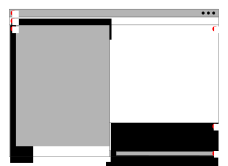
\includegraphics[width=\linewidth]{build/gui/main_view_initial.png}}
\captionof{figure}{Hauptfenster unmittelbar nach dem Starten des Programms}
\end{minipage}

Das Hauptfenster besteht aus der Fensterleiste (A), der Menüleiste (1), dem Editor (2), der Visualisierungsbox (3), der Konsole (4) und dem Eingabefeld (5).
Dabei ist die Fensterleiste kein Bestandteil des Programms; sie ist von der graphischen Oberfläche des Betriebssystems vorgegeben.
Das Eingabefeld ist deaktiviert (angedeutet durch die graue Färbung), da noch kein Prolog-Programm geparst wurde.

\subsubsection{\enquote{Datei}-Menü}

\begin{minipage}{\linewidth}
\makebox[\linewidth]{
    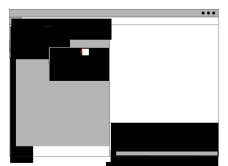
\includegraphics[width=\linewidth]{build/gui/main_view_filemenu.png}}
\captionof{figure}{Hauptfenster mit ausgewähltem \enquote{Datei}-Menü}
\end{minipage}

Das \enquote{Datei}-Menü (1) hat die Einträge \enquote{Neu}, \enquote{Öffnen}, \enquote{Speichern}, \enquote{Speichern als...}, \enquote{Zuletzt verwendet} und \enquote{Beenden}.
\enquote{Neu}, \enquote{Öffnen} und \enquote{Speichern} führen die jeweiligen Funktionen aus.
Während \enquote{Speichern} nur bei neu angelegten Prolog-Programmen einen Auswahldialog anzeigt, zeigt \enquote{Speichern als...} immer einen Auswahldialog an.
\enquote{Beenden} beendet das Programm.
\enquote{Zuletzt verwendet} enthält eine Liste von bis zu fünf zuletzt verwendeten Programmen (2).

\subsubsection{Geöffnete Datei}

\begin{minipage}{\linewidth}
\makebox[\linewidth]{
    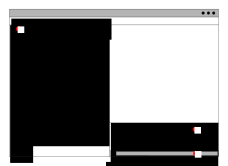
\includegraphics[width=\linewidth]{build/gui/main_view_opened.png}}
\captionof{figure}{Hauptfenster nach dem Öffnen des Beispielprogramms}
\end{minipage}

Nach dem Öffnen des Beispielprogramms wird dessen Inhalt im Editor angezeigt (1).
Die Konsole gibt eine entsprechende Meldung aus (2).
Das Eingabefeld bleibt weiterhin deaktiviert (3).

\subsubsection{Parsen fehlgeschlagen}

\begin{minipage}{\linewidth}
\makebox[\linewidth]{
    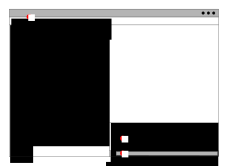
\includegraphics[width=\linewidth]{build/gui/main_view_parse_fail.png}
}
\captionof{figure}{Hauptfenster nach Klick auf \enquote{Parsen}, mit inkorrektem Prolog-Programm}
\end{minipage}

Klickt der Nutzer auf \enquote{Parsen} (1), versucht der Parser das Prolog-Programm im Editor zu verarbeiten.
Stößt er dabei auf Fehler, wird eine Fehlermeldung in der Konsole angezeigt (2).
Das Eingabefeld bleibt weiterhin deaktiviert (3).

\subsubsection{Parsen erfolgreich}

\begin{minipage}{\linewidth}
\makebox[\linewidth]{

\includegraphics[width=\linewidth]{build/gui/main_view_parse_success.png}
}
\captionof{figure}{Hauptfenster nach Klick auf \enquote{Parsen}, mit korrektem Prolog-Programm}
\end{minipage}

Klickt der Nutzer auf \enquote{Parsen} (1), versucht der Parser das Prolog-Programm im Editor zu verarbeiten.
Treten dabei keine Fehler auf, wird eine entsprechende Meldung in der Konsole angezeigt (2).
Das Eingabefeld wird aktiviert; der Nutzer kann jetzt Abfragen eingeben (3).

\subsubsection{Fehlerhafte Abfrage}

\begin{minipage}{\linewidth}
\makebox[\linewidth]{

\includegraphics[width=\linewidth]{build/gui/main_view_question_fail.png}
}
\captionof{figure}{Hauptfenster nach fehlerhafter Abfrage im Eingabefeld}
\end{minipage}

Gibt der Nutzer eine Abfrage im Eingabefeld ein (1), versucht der Parser, diese Eingabe zu einem einzelnen Ziel zu verarbeiten.
Stößt er dabei auf Fehler, wird eine Fehlermeldung in der Konsole angezeigt (2).

\subsubsection{Erfolgreiche Abfrage}

\begin{minipage}{\linewidth}
\makebox[\linewidth]{
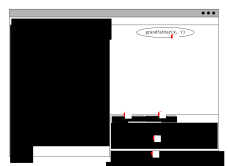
\includegraphics[width=\linewidth]{build/gui/main_view_visualisation_root.png}
}
\captionof{figure}{Hauptfenster nach Eingabe einer Abfrage}
\end{minipage}

Gibt der Nutzer eine Abfrage (1) im Eingabefeld ein, versucht der Parser, diese Eingabe zu einem einzelnen Ziel zu verarbeiten.
Treten dabei keine Fehler auf, wird eine Meldung in der Konsole angezeigt (2) und die Visualisierung der Abarbeitung dieser Abfrage gestartet (3).
Eine Leiste mit Schaltflächen, die zur Steuerung der Visualisierung dienen, wird angezeigt.
Die Schaltfäche \enquote{Nächster Schritt} (4) bewirkt die Ausführung und Visualisierung des nächsten Schrittes.
Die Schaltflächen \enquote{+} und \enquote{-} (5) dienen zum Zoomen in der Visualisierung.

\subsubsection{Lösung gefunden}

\begin{minipage}{\linewidth}
\makebox[\linewidth]{
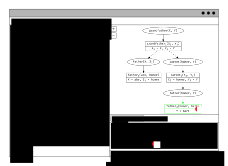
\includegraphics[width=\linewidth]{build/gui/main_view_solution_found.png}
}
\captionof{figure}{Eine Lösung wurde gefunden}
\end{minipage}

Wurde ein Lösung für die Abfrage gefunden (1), wird eine Meldung in der Konsole angezeigt (2).

\subsubsection{Keine weiteren Lösungen}

\begin{minipage}{\linewidth}
\makebox[\linewidth]{
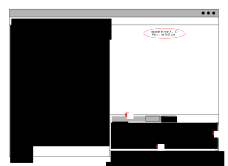
\includegraphics[width=\linewidth]{build/gui/main_view_no_more_solutions.png}
}
\captionof{figure}{Es gibt keine weiteren Lösungen mehr}
\end{minipage}

Gibt es keine weiteren Lösungen mehr, wird eine Meldung (1) in der Konsole angezeigt und die Schaltfläche \enquote{Nächster Schritt} wird deaktiviert (2).

Dieser Fall tritt ein, wenn der Interpreter einen Rückschritt vom eingegeben Ziel auszuführen versucht.
In diesem Fall gibt es keine Fakten mehr, die mit dem Ziel unifizierbar sind.
Unabhängig davon, ob es per se keine Lösungen gibt oder schon Lösungen gefunden wurden, wird die Meldung \enquote{Keine weiteren Lösungen.} angezeigt.

In diesem Entwurf ist außerdem der Scrollbalken gezeigt (3).
Dieser wird neben der Konsole eingeblendet, wenn der angezeigt Text nicht mehr hineinpasst.
Dies gilt auch für den Editor.

\subsection{Kannkriterien}

Jeder der folgenden Entwürfe beinhaltet \emph{ein} Kannkriterium.

\subsubsection{Schaltfläche \enquote{Vorheriger Schritt}}

\begin{minipage}{\linewidth}
\makebox[\linewidth]{
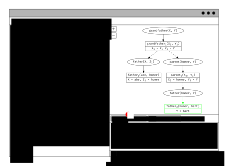
\includegraphics[width=\linewidth]{build/gui/main_view_previous_step.png}
}
    \captionof{figure}{Die Schaltfläche \enquote{vorheriger Schritt}}
\end{minipage}

\begin{minipage}{\linewidth}
\makebox[\linewidth]{
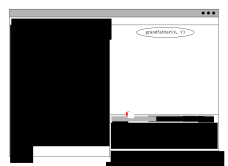
\includegraphics[width=\linewidth]{build/gui/main_view_previous_step_disabled.png}
}
\captionof{figure}{Interpreter beim ersten Schritt; die Schaltfläche \enquote{Vorheriger Schritt} ist deaktiviert}
\end{minipage}

Die Schaltfläche \enquote{Vorheriger Schritt} (1) erlaubt es dem Nutzer, den Zustand vor dem aktuellen Schritt zu betrachten.
Die Schaltfläche kann so lange betätigt werden, bis der Nutzer beim ersten Schritt angelangt ist.
Ist der Nutzer beim ersten Schritt angelangt, wird die Schaltfläche deaktiviert.

\subsubsection{Ausführung bis zur nächsten Lösung}

\begin{minipage}{\linewidth}
\makebox[\linewidth]{
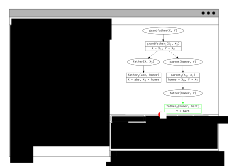
\includegraphics[width=\linewidth]{build/gui/main_view_next_solution.png}
}
\captionof{figure}{Die Schaltfläche \enquote{Nächste Lösung}}
\end{minipage}

\begin{minipage}{\linewidth}
\makebox[\linewidth]{
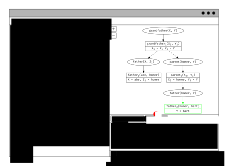
\includegraphics[width=\linewidth]{build/gui/main_view_abort.png}
}
\captionof{figure}{Die Schaltfläche \enquote{Abbrechen}}
\end{minipage}

Die Schaltfläche \enquote{Nächste Lösung} (1) lässt den Interpreter automatisch Schritte ausführen, bis eine Lösung gefunden wurde oder keine Unifikation der Abfrage mehr möglich ist.
Betätigt der Nutzer die Schaltfläche, wird sie hervorgehoben und ihr Text in \enquote{Abbrechen} geändert.
Betätigt der Nutzer die Schaltfläche erneut, wird der Interpreter unterbrochen und der letzte vollständig berechnete Schritt angezeigt.

\subsection{Visualisierung}

Um die Visualisierungsbeispiele besser darzustellen zu können, wurden sie hier ohne die graphische Oberfläche des Programms eingefügt.
Die visualisierte Abfrage ist \texttt{grandfather(X, Y)} im Beispielprogramm.

\subsubsection{Wurzel}

\begin{minipage}{\linewidth}
\makebox[\linewidth]{
\includegraphics[width=\linewidth]{build/visualisation/01_root.png}
}
\captionof{figure}{Wurzel des Visualisierungsbaumes}
\end{minipage}

Die Wurzel des Visualisierungsbaumes stellt die eingegebene Abfrage dar.

\subsubsection{Fehlgeschlagene Unifikation}

Im nächsten Schritt versucht der Interpreter die Unifikation von \texttt{grandfather(X, Y)} mit dem Fakt \texttt{father(abe, homer)}.
Diese schlägt fehl.

\begin{minipage}{\linewidth}
\makebox[\linewidth]{
\includegraphics[width=\linewidth]{build/visualisation/02_root_fail.png}
}
\captionof{figure}{Eine fehlgeschlagene Unifikation}
\end{minipage}

Die Visualisierung stellt zu unifizierende Ziele als Runde Knoten dar.
Unifikationen werden in  Rechtecken dargestellt, die in zwei weitere Rechtecke aufgeteilt sind.
Dabei enthält jede Unifikation im oberen Rechteck den Fakt, mit dem unifiziert werden soll.
Fehlgeschlagene Unifikationen enthalten im unteren Rechteck den Satz \enquote{Unifikation fehlgeschlagen:} und den Grund des Fehlschlags.
Außerdem sind sie rot eingefärbt.

\subsubsection{Erfolgreiche Unifikation und Teilziele}

In den weiteren Schritten schlagen die Unifikationen von \texttt{grandfather(X, Y)} mit \texttt{father(homer, bart)}, \texttt{father(homer, lisa)} und \texttt{mother(marge, bart)} fehl.
Die Unifikation mit der Regel \texttt{grandfather(X, Y)} ist erfolgreich.
Dabei werden die Variablennamen durch neue, eindeutige Namen ersetzt um Konflikte zu vermeiden.

\begin{minipage}{\linewidth}
\makebox[\linewidth]{
\includegraphics[width=\linewidth]{build/visualisation/03_root_success.png}
}
\captionof{figure}{Eine erfolgreiche Unifikation mit Einfügung der Teilziele}
\end{minipage}

Erfolgreiche Unifikationen enthalten im unteren Rechteck die resultierenden Substitutionen.
Außerdem sind sie grün eingefärbt.

War eine Unifikation mit einer Regel erfolgreich, so werden ihre Teilziele als neue Ziele, also runde Knoten, zum Graphen hinzugefügt.
Die Substitutionen werden in den Teilzielen angewendet und hervorgehoben.
Die Unifikation und ihre Teilziele werden durch gestrichelte Kanten verbunden.
Dadurch werden im Baum die Fälle \enquote{Ziel wurde unifiziert mit} und \enquote{Ziel ist Teilziel von Regel} unterschieden.

\subsubsection{Erfolgreiche Unifikation mit rückwirkender Substitution}

Im nächsten Schritt steigt der Interpreter in die Teilziele ab und versucht, von links nach rechts diese zu unifizieren.

\begin{minipage}{\linewidth}
\makebox[\linewidth]{
\includegraphics[width=\linewidth]{build/visualisation/04_subgoal_father_success.png}
}
\captionof{figure}{Eine erfolgreiche Unifikation mit mit rückwirkender Substitution}
\end{minipage}

In diesem Beispiel hat der gefundene Fakt keine Teilziele.
Trotzdem müssen die Substitutionen in der restlichen Teilzielen angewendet werden.
Die angewendeten Substitutionen werden dabei in den betreffenden Zielen hervorgehoben.

\subsubsection{Backtracking}

Hier wurden einige Schritte übersprungen.
Das zweite Teilziel wurde mit der ersten Definition von \texttt{parent(X, Y)} unifiziert.
Diese hat als Teilziel \texttt{mother(X, Y)}.
Mit der Belegung \texttt{X = homer} gibt es dafür aber keine Lösung.
Der Interpreter muss also nach einer alternativen Definition von \texttt{parent} suchen und dazu zurückspringen (\enquote{Backtracking}).

\begin{minipage}{\linewidth}
\makebox[\linewidth]{
\includegraphics[width=\linewidth]{build/visualisation/09_mother_backtrack.png}
}
\captionof{figure}{Rücksprung nachdem ein Ziel nicht erfüllbar ist}
\end{minipage}

Ein Rücksprung wird durch eine aus Punkten bestehende, rot eingefärbte Kante dargestellt.
Das nicht erfüllbare Teilziel wird ebenfalls rot eingefärbt und mit dem Text \enquote{Nicht erfüllbar!} ergänzt.

\section{Glossar}

\subsection{Allgemein}

\textbf{Programm}:
Das vorgestellte VIPER-Programm. Dies ist zu unterscheiden von Prolog-Programmen.

\textbf{Prolog-Programm}:
Prolog-Quelltext in Form von Dateien auf einem Speichermedium. Dies ist zu unterscheiden von dem Programm im Sinne des VIPER-Programms.

\subsection{Prolog-interne Begriffe}
\textbf{Fakt}:
Aussage, welche als wahr angenommen wird.

Im Kontext von Prolog: eine Regel ohne Teilziele.

\textbf{Regel}:
Vorgeschriebene Folgerungen. Regeln können bspw. festsetzen, dass aus dem Fakt, dass jemand ein Elternteil ist, folgt, dass dieser Elternteil entweder Mutter oder Vater sein muss.

\textbf{Identifier}:
Wort, beginnend mit einem Kleinbuchstaben und fortsetzend mit Groß- und Kleinbuchstaben sowie Zahlen.

\textbf{Variable}:
Platzhalter. Erlaubt das allgemeine Beschreiben von Regeln. Können für einen beliebigen Term stehen.

\textbf{Funktor}:
Sammelbegriff für Identifier, welche für sich allein stehen oder eine Liste an Termen auswerten.

\textbf{Ziel}:
Sammelbegriff für Funktoren, Vergleiche von Termen über den \enquote{\texttt{=}}-Operator, Arithmetik oder den \enquote{Cut}-Operator (\texttt{!}).

\textbf{Term}:
Sammelbegriff für Funktoren, Variablen oder Zahlen.

\textbf{Standardbibliothek}:
Voreingestellte Regeln, welche automatisch bei der Verarbeitung durch den Parser angefügt werden können.

\textbf{Abfrage}:
Ziel, welches ausgewertet werden soll. Das Ergebnis der Auswertung kann eine Menge an Lösungen oder eine Ja-Nein-Antwort sein.

\textbf{Parser}:
Auswertungsmechanismus für Prolog-Programme, der diese in ein für die Weiterverarbeitung geeignetes Format bringt und auf syntaktische Fehler prüft.

\textbf{Interpreter}:
Ausführungsmechanismus für Abfragen. Nachdem sowohl das zugrunde liegende Prolog-Programm als auch die Abfrage durch den Parser verarbeitet wurden, findet eine Auswertung der genannten Abfrage statt. Diese Auswertung wird schrittweise abgearbeitet und ist durch das Programm verfolgbar.

\textbf{Schritt}:
Nächste Operation, die zur Auswertung einer Abfrage nötig ist.

\textbf{Zustand}:
Ergebnis der bisher durchgeführten Schritte.

\textbf{Zustandsunterschied}:
Schritte zwischen zwei Zuständen.

\textbf{Rekursion}:
Eine Regel wird rekursiv genannt, wenn sie selbst eines ihrer Teilziele ist.

\textbf{Arithmetik}:
Auswertung mathematischer Operationen (bspw. Summen, Differenzen etc.).

\subsection{Begriffe der Bedienoberfläche}
\textbf{Öffnen}:
Lesen eines ausgewählten Prolog-Programms von einem verbundenen Speichermedium in das Programm. Dies entspricht der Übertragung des Textes aus der gewählten Datei in den Editor.

\textbf{Speichern}:
Schreiben einer Prolog-Programmdatei in ein Zielverzeichnis auf einem verbundenen Speichermedium. Es werden ausschließlich Prolog-Programme gespeichert, andere Schreibvorgänge auf Speichermedien fallen unter den Begriff Export.

\textbf{Export}:
Schreiben von Bild-Dateien oder LaTeX-Quellcode in ein Zielverzeichnis auf einem verbundenen Speichermedium. Das Schreiben von Prolog-Programmen auf ein Speichermedium wird nicht als Export, sondern als Speichern bezeichnet.

\textbf{Editor}:
Element der graphischen Oberfläche, welches Eingabe und Bearbeitung von angezeigtem Text ermöglicht.

\textbf{Konsole}:
Element der graphischen Oberfläche. Die Konsole ist nur lesbar und dient der Ausgabe von Ergebnissen einer Abfrage sowie anderen Meldungen. 

\textbf{Eingabefeld}:
Element der graphischen Oberfläche. Das Eingabefeld dient zur Eingabe von Abfragen. Es ist nur dann aktiviert, wenn ein gültiges Prolog-Programm eingegeben und geparst wurde.

\textbf{Graph}:
Struktur bestehend aus Knoten und Kanten.

\textbf{Visualisierung}:
Navigierbarer Graph, welcher den Ablauf der Interpretation einer Abfrage im Kontext eines gegebenen Prolog-Programms aufzeigt.

\textbf{Zoom}:
Vergrößerung oder Verkleinerung eines Bildausschnitts.

\textbf{Syntax / Syntax-Highlighting}:
Eine Syntax entspricht einem Regelsystem, welches valide Zeichenkombinationen festlegt. Die Prolog-Syntax ist fest definiert und beschreibt den Aufbau valider Prolog-Programme. Syntax-Highlighting entspricht einer visuellen Unterstützung durch Schrifteffekte und -farben, um die Syntax ersichtlicher zu machen (Einfärbung von zusammengehörigen Klammern etc.).

\textbf{GUI / GUI-Element}:
Das GUI entspricht der graphischen Benutzeroberfläche (graphical user interface). Das GUI ist zusammengesetzt aus diversen GUI-Elementen innerhalb eines Fensters (bspw. dem Editor).

\textbf{Menüleiste}:
Element der graphischen Oberfläche. Bietet über Text-Menüs Zugriff auf Funktionen wie Speichern und Öffnen.

\textbf{Dialog}:
Fenster zur Meldung einer Nachricht (Warnungs- oder Fehler-Dialog) oder Anfrage (bspw. Bestätigungs-Dialog).

\textbf{Formatierung}:
Vorgegebener Stil bzgl. der Setzung von Leerzeichen und Umbrüchen. Zu unterscheiden von Syntax, da Formatierung keinen Einfluss auf die Validität des Programms hat.

\newpage
\section{Anhang}

\subsection{Formatiertes simpsons.pl Beispielprogramm}

\begin{lstlisting}
father(abe, homer).
father(homer, bart).
father(homer, lisa).
mother(marge, bart).

grandfather(X, Y) :-
  father(X, Z), parent(Z, Y).

parent(X, Y) :-
  mother(X, Y).

parent(X, Y) :-
  father(X, Y).
\end{lstlisting}

\subsection{Unformatiertes simpsons.pl Beispielprogramm}

\begin{lstlisting}
father(abe, homer). father(homer, bart).
father(homer, lisa). mother(marge, bart).

grandfather(X, Y) :-
father(X, Z), parent(Z, Y).

parent(X, Y) :- mother(X, Y).

parent(X, Y) :- father(X, Y).
\end{lstlisting}

\end{document}
